\chapter{Security Analysis}
\label{sec:security_analyse}

% Ist das zentrale Kapitel der Arbeit. Hier werden das Ziel sowie die
% eigenen Ideen, Wertungen, Entwurfsentscheidungen vorgebracht. Es kann
% sich lohnen, verschiedene Möglichkeiten durchzuspielen und dann
% explizit zu begründen, warum man sich für eine bestimmte entschieden
% hat. Dieses Kapitel sollte - zumindest in Stichworten - schon bei den
% ersten Festlegungen eines Entwurfs skizziert werden.
% Es wird sich aber in einer normal verlaufenden
% Arbeit dauernd etwas daran ändern. Das Kapitel darf nicht zu
% detailliert werden, sonst langweilt sich der Leser. Es ist sehr
% wichtig, das richtige Abstraktionsniveau zu finden. Beim Verfassen
% sollte man auf die Wiederverwendbarkeit des Textes achten.

% Plant man eine Veröffentlichung aus der Arbeit zu machen, können von
% diesem Kapitel Teile genommen werden. Das Kapitel wird in der Regel
% wohl mindestens 8 Seiten haben, mehr als 20 können ein Hinweis darauf
% sein, daß das Abstraktionsniveau verfehlt wurde.

%\ldots design \ldots

%\todo{write design}
This chapter aims to analyze the potential vulnerabilities in Quark~\cite*{quark}, through which an adversary can obtain sensitive data of an application. The first section defines the threat model (Section~\ref{sec:Threat_model}). 
Subsequently, this chapter scrutinizes Quark's security from the perspective of the Open Container Initiative (OCI) interface~\cite*{oci-runtime-spec} (Section~\ref{sec:security_analysis}).

\section{Threat Model}
\label{sec:Threat_model}
We employ the OWASP application threat modeling methodology\cite*{OWASP_Threat_Modeling} to create a threat model comprising four aspects: actors, assets, external dependencies, and attack surface. 

\textbf{Actors.} Our model involves the cloud provider and the tenant. The cloud provider is accountable for providing the hardware and software necessary for running and orchestrating applications. However, the tenant distrusts the cloud provider in the 
context of confidential computing. Therefore, the software components within the cloud infrastructure like Kubernetes control plane\cite*{k8s}, containerd\cite*{containerd}, and hypervisor (Qvisor) are untrusted.

\textbf{Assets.} Our objective is to secure the Kubernetes workload (application) itself, i.e., preserving the integrity of the application binary and its dependencies, maintaining the confidentiality and integrity of the application's data during runtime, and protecting the secrets provided to the application by its owner.

\textbf{External Dependencies.} We assume that the guests, including Qkernel and workloads, operate within a \acrshort{TEE}. This prevents malicious hypervisor (Qvisor) or powerful cloud operators from accessing the workload's sensitive 
data through guest memory and registers. Furthermore, we exclude attacks related to denial of service~\cite*{DOS_ATTACK}, side channels~\cite*{217454}, networks, or file systems.


\textbf{Attack Surface.} We focus on attacks occurring on the OCI interface~\cite*{oci-runtime-spec}. As the management of workloads is the cloud provider's responsibility, it must have a means of accessing workloads for orchestration, even if the 
workloads are running within a \acrshort{TEE}. Although the OCI runtime specification offers this possibility, it exposes a new attack surface for an adversary to probe workloads' secrets. Additionally, since the OCI  implementation in the guest interacts with 
the host through the Hypercall, Qcall, or Ucall interface, we also mention what specific call an adversary use to launch attacks. The workflow of Hypercall, Qcall, or Ucall can be found in Section~\ref{sec:Quark}.


\section{Security Analysis}
\label{sec:security_analysis}
This section provides a security analysis of the OCI runtime interfaces~\cite*{oci-runtime-spec} implemented within Quark. Notably, Qlib serves solely as a development concept since its code is incorporated into the Qkernel and Qvisor binaries 
during the compilation. Therefore, the following sections use Qkernel and Qvisor to refer to the respective binaries containing the Qlib code.

The subsequent sections examine the potential pitfalls of the OCI implementation in Quark from seven perspectives:

\begin{itemize}
  \item Application secrets deployment.
  \item Handling STDIO of guest user space process.
  \item Command execution and terminal allocation.
  \item Para-virtualized file system sharing.
  \item Guest system call.
  \item Guest kernel arguments.
  \item Guest logging system. 
\end{itemize}

A summary of the vulnerabilities we found is available in Section~\ref{sec:security_summarize}. Chapter~\ref{sec:design} further proposes mechanisms to mitigate these vulnerabilities.


\subsection{Application Secrets Deployment}
\begin{figure}[htp]
    \centering
    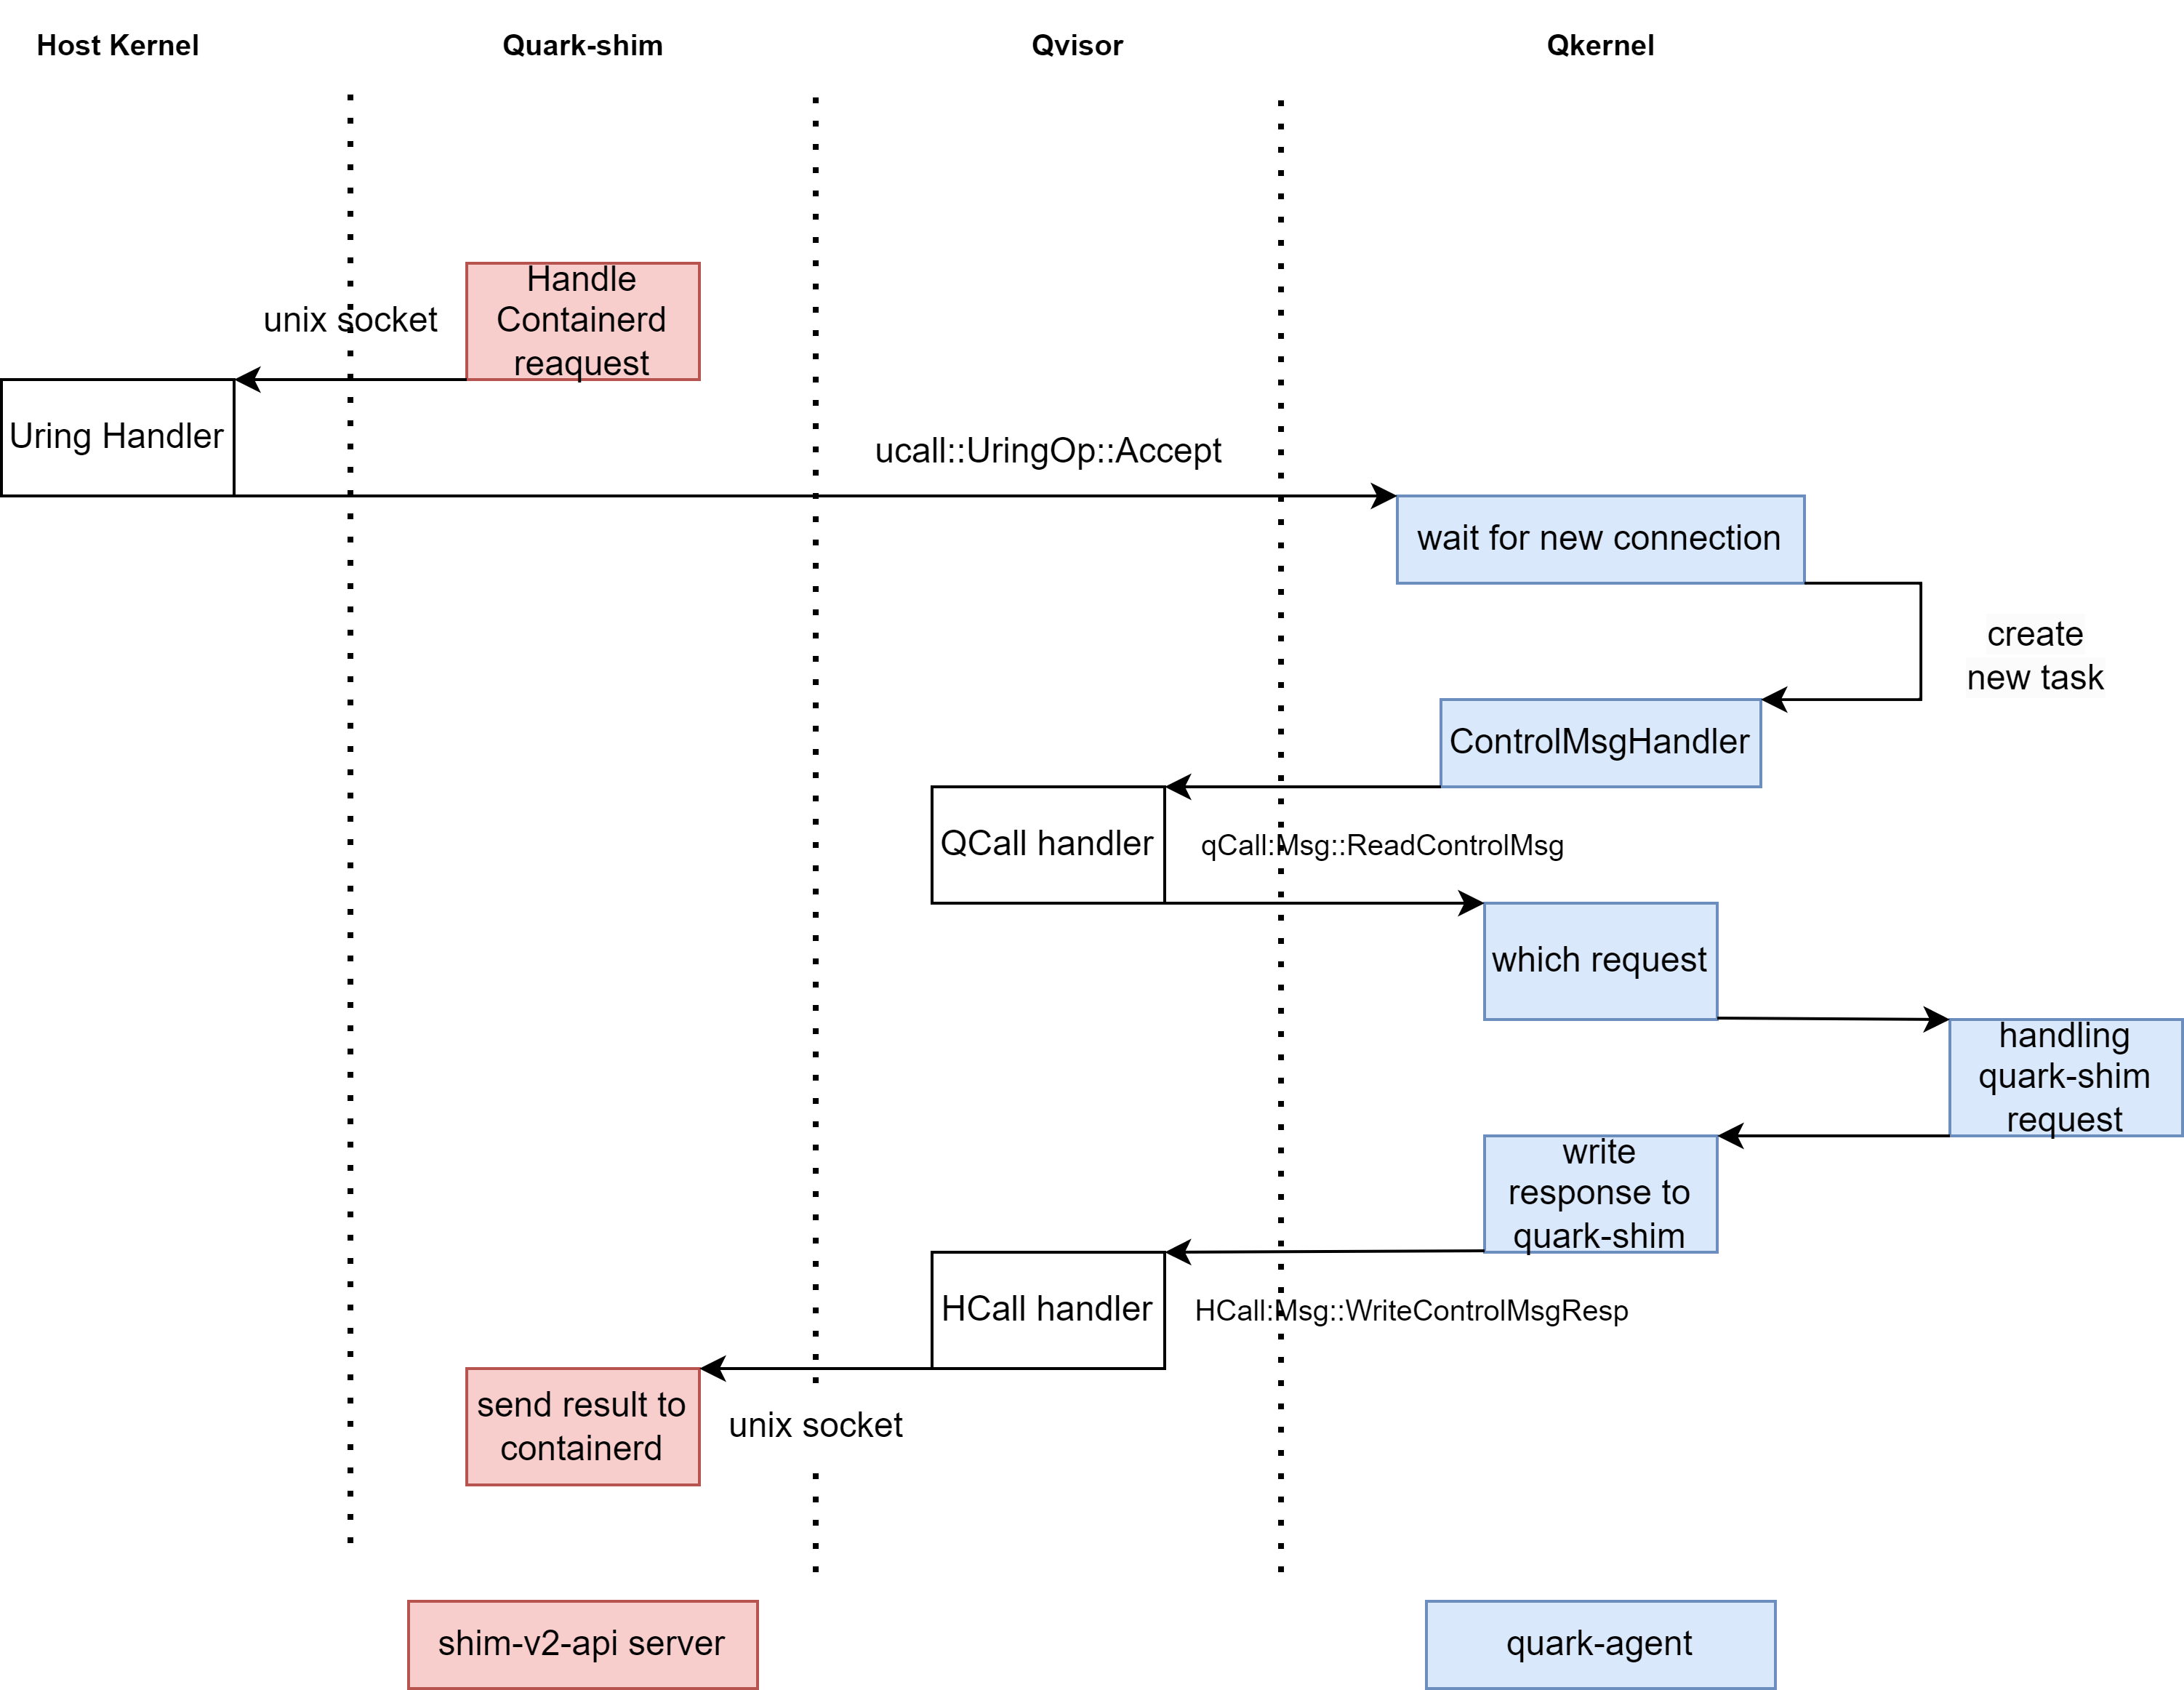
\includegraphics[width=0.8\textwidth]{images/quark-agent-work-flow.png}
    \caption[Quark Agent Workflow]{Quark agent workflow}
    \label{fig:quark_agent_work_flow}
\end{figure}


\textbf{Untrusted Kubernetes and the Quark Shim manage and deploy application secrets}. 
These secrets may be injected into the application through command line arguments, mounted files, or environment variables. When deploying the application, Containerd~\cite*{containerd} generates an application 
bundle and transmits it via the shim v2 API~\cite*{shim_v2} to the shim-v2-API server in the Quark Shim.  As discussed in Section~\ref{sec:back_oci_runtime_spec}, this bundle contains the rootfs of the application along with an OCI-compatible configuration file~\cite*{oci-runtime-spec}. Quark Shim creates the root filesystem for the container on the host side, 
mounts the file type secret, and passes the process specification via Unix socket. The specification contains metadata for creating a process in the guest, including command line arguments, environment variables, the type of STDIO (interactive or non-interactive IO), and the host file descriptor 
for transmitting data from/to the process STDIO. Upon receiving the specification, the Quark agent in the Qkernel will create an application process accordingly.  The workflow is shown in Figure~\ref{fig:quark_agent_work_flow}.

Quark-agent operates as a socket server accepting connection requests from the Quark Shim through Ucall::Uringop::accept(). These requests include creating and deleting application processes, creating an exec process, etc. Upon receiving a request from Quark Shim to create an application (EXEC) 
 process, the Uringop::accept returns a host file descriptor that contains the process specification. As the agent in the Qkernel cannot read its contents directly, it employs Qcall:Msg::ReadControlMsg to request the Qvivor to read the file descriptor and return the specification. Based on the 
 specification, Quark-agent creates a guest user process. Specifically, the command line arguments and the environment variables are pushed to the process stack, and the STDIO of the process is set accordingly to the type of STDIO specified in the specification. Further details about the process’s 
 STDIO can be found in section~\ref{sec:security_analyse_STDIO}.

It is imprudent to let Kubernetes~\cite*{k8s} manage application secrets and deploy them through untrusted Containerd~\cite*{containerd} and Quark Shim. In particular, individuals with access to the cluster can use the kubectl to view or modify the secrets. Additionally, an adversary can manipulate Containerd 
and Quark Shim to tamper with the application secrets during application deployment. Besides, when Quark-agent uses the Qcall interface to request Qvisor to read the process specification, Qvisor could potentially steal or modify these secrets. To this end, we suggest offloading secret deployment and management 
from Kubernetes, Quark Shim, and Qvisor. For a detailed explanation of the mitigation, please refer to section~\ref{sec:design_Secret_Uploading}.

\subsection{Guest User Space Process STDIO}
\label{sec:security_analyse_STDIO}

The Quark agent loads the corresponding binary and initiates a guest user-space process for handling the request, such as creating an application or executing a command (kubectl exec)~\cite*{k8s}. Thus, Quark handles the application process STDIO in the same way as it handles the exec process STDIO. For instance, 
when Containerd~\cite*{containerd} wishes to create an EXEC process in Qkernel, three named pipes are created for the process’s standard input, output, and error. These are then passed to Quark Shim with other metadata. Quark Shim then employs these data to create the  EXEC request’s process 
specification.

\begin{figure}[ht] 
    \begin{subfigure}[b]{0.5\linewidth}
      \centering
      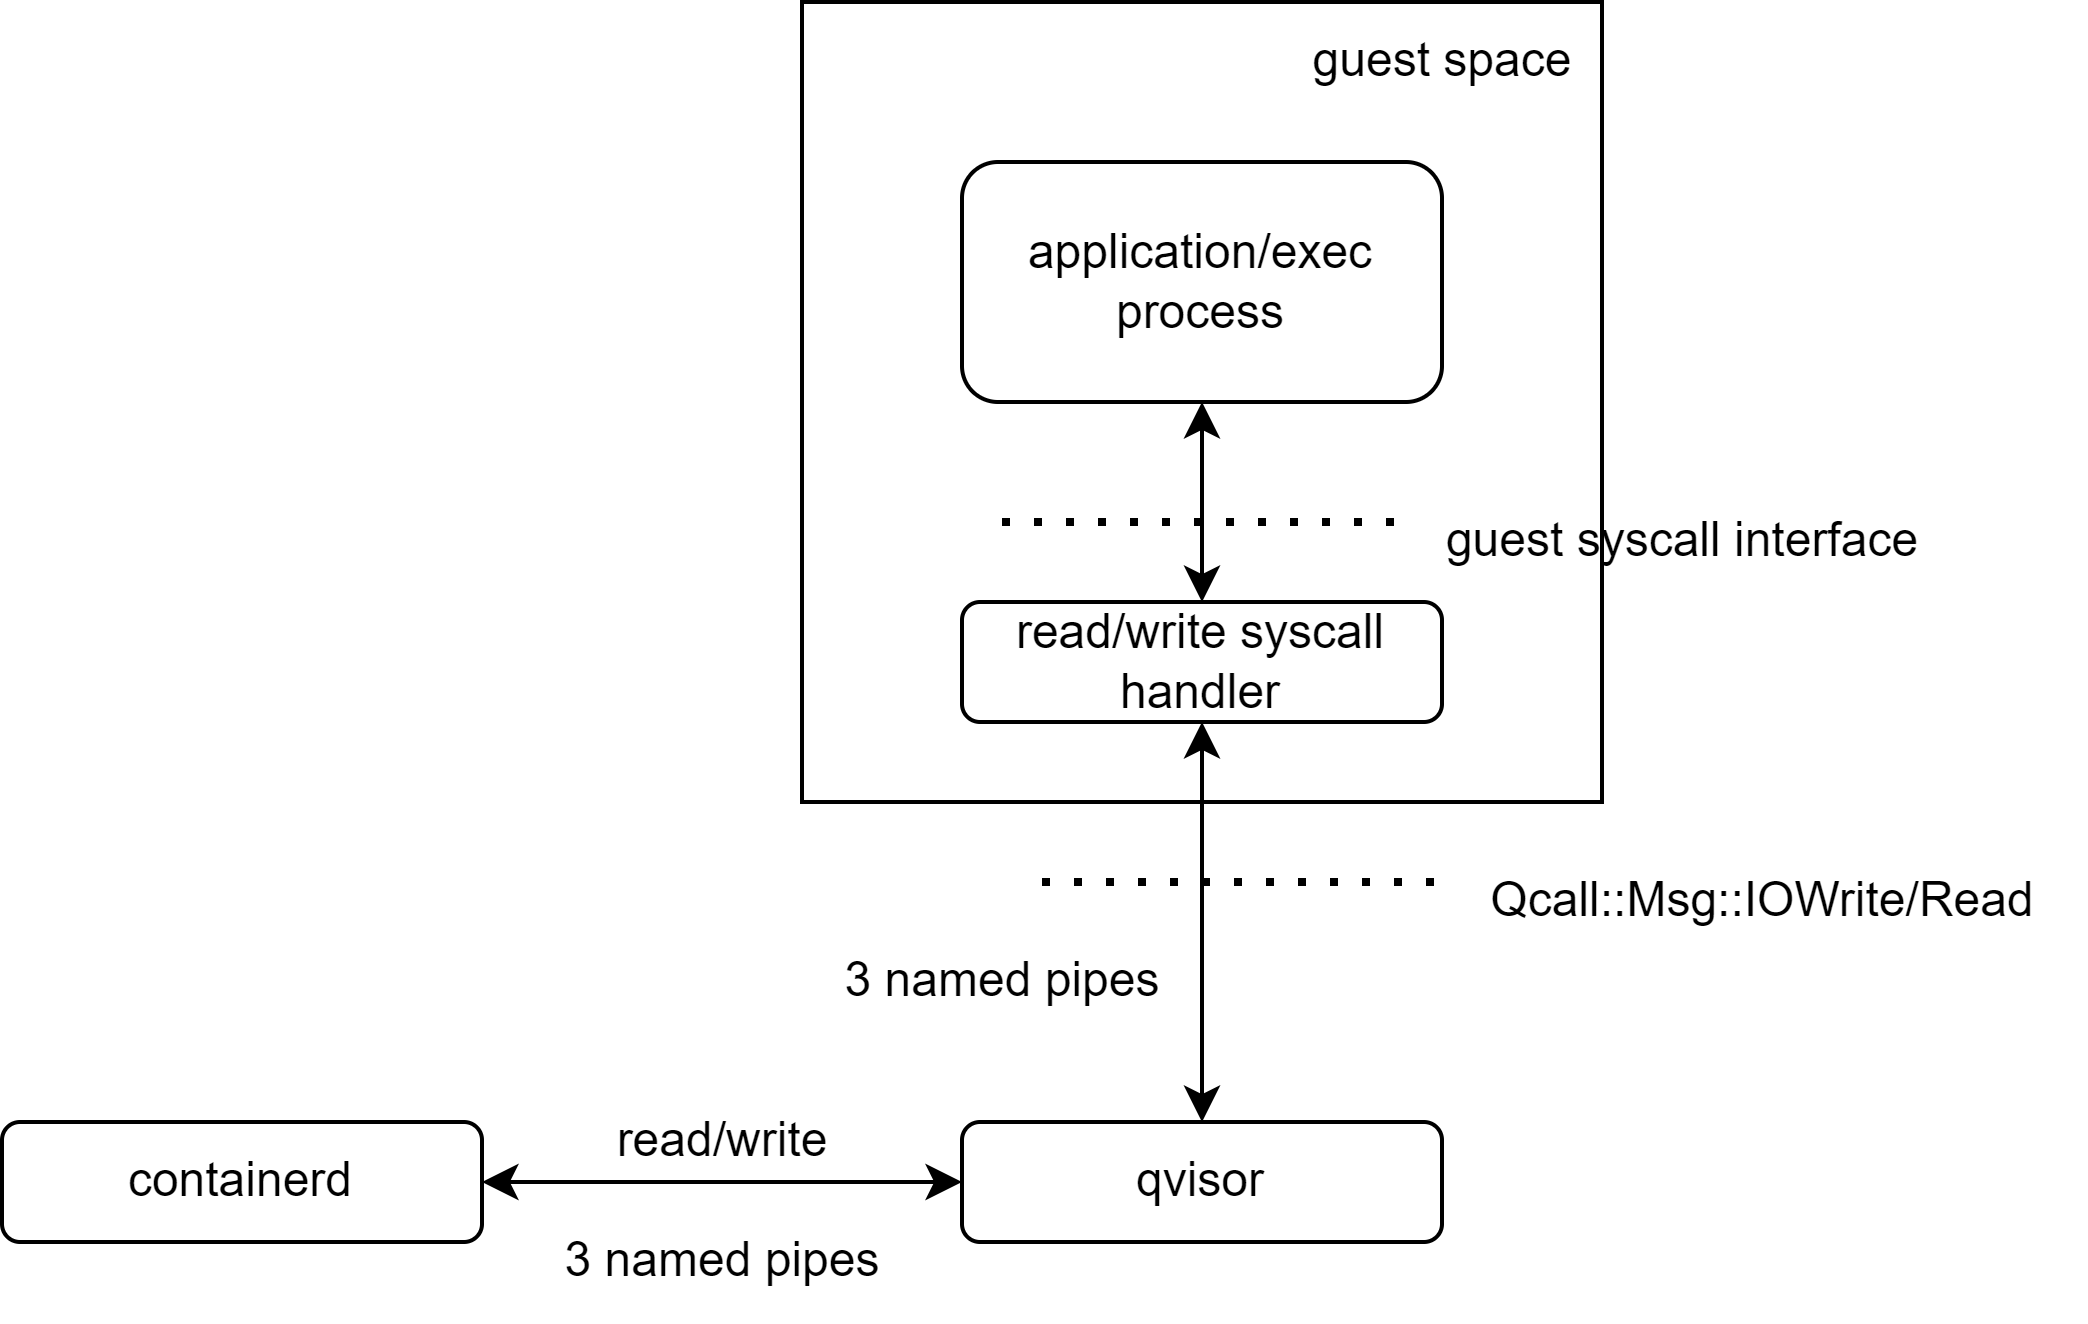
\includegraphics[width=0.9\linewidth]{images/normorl_io.png} 
      \caption{Normal IO} 
      \label{fig1:a} 
      \vspace{4ex}
    \end{subfigure}%% 
    \begin{subfigure}[b]{0.5\linewidth}
      \centering
      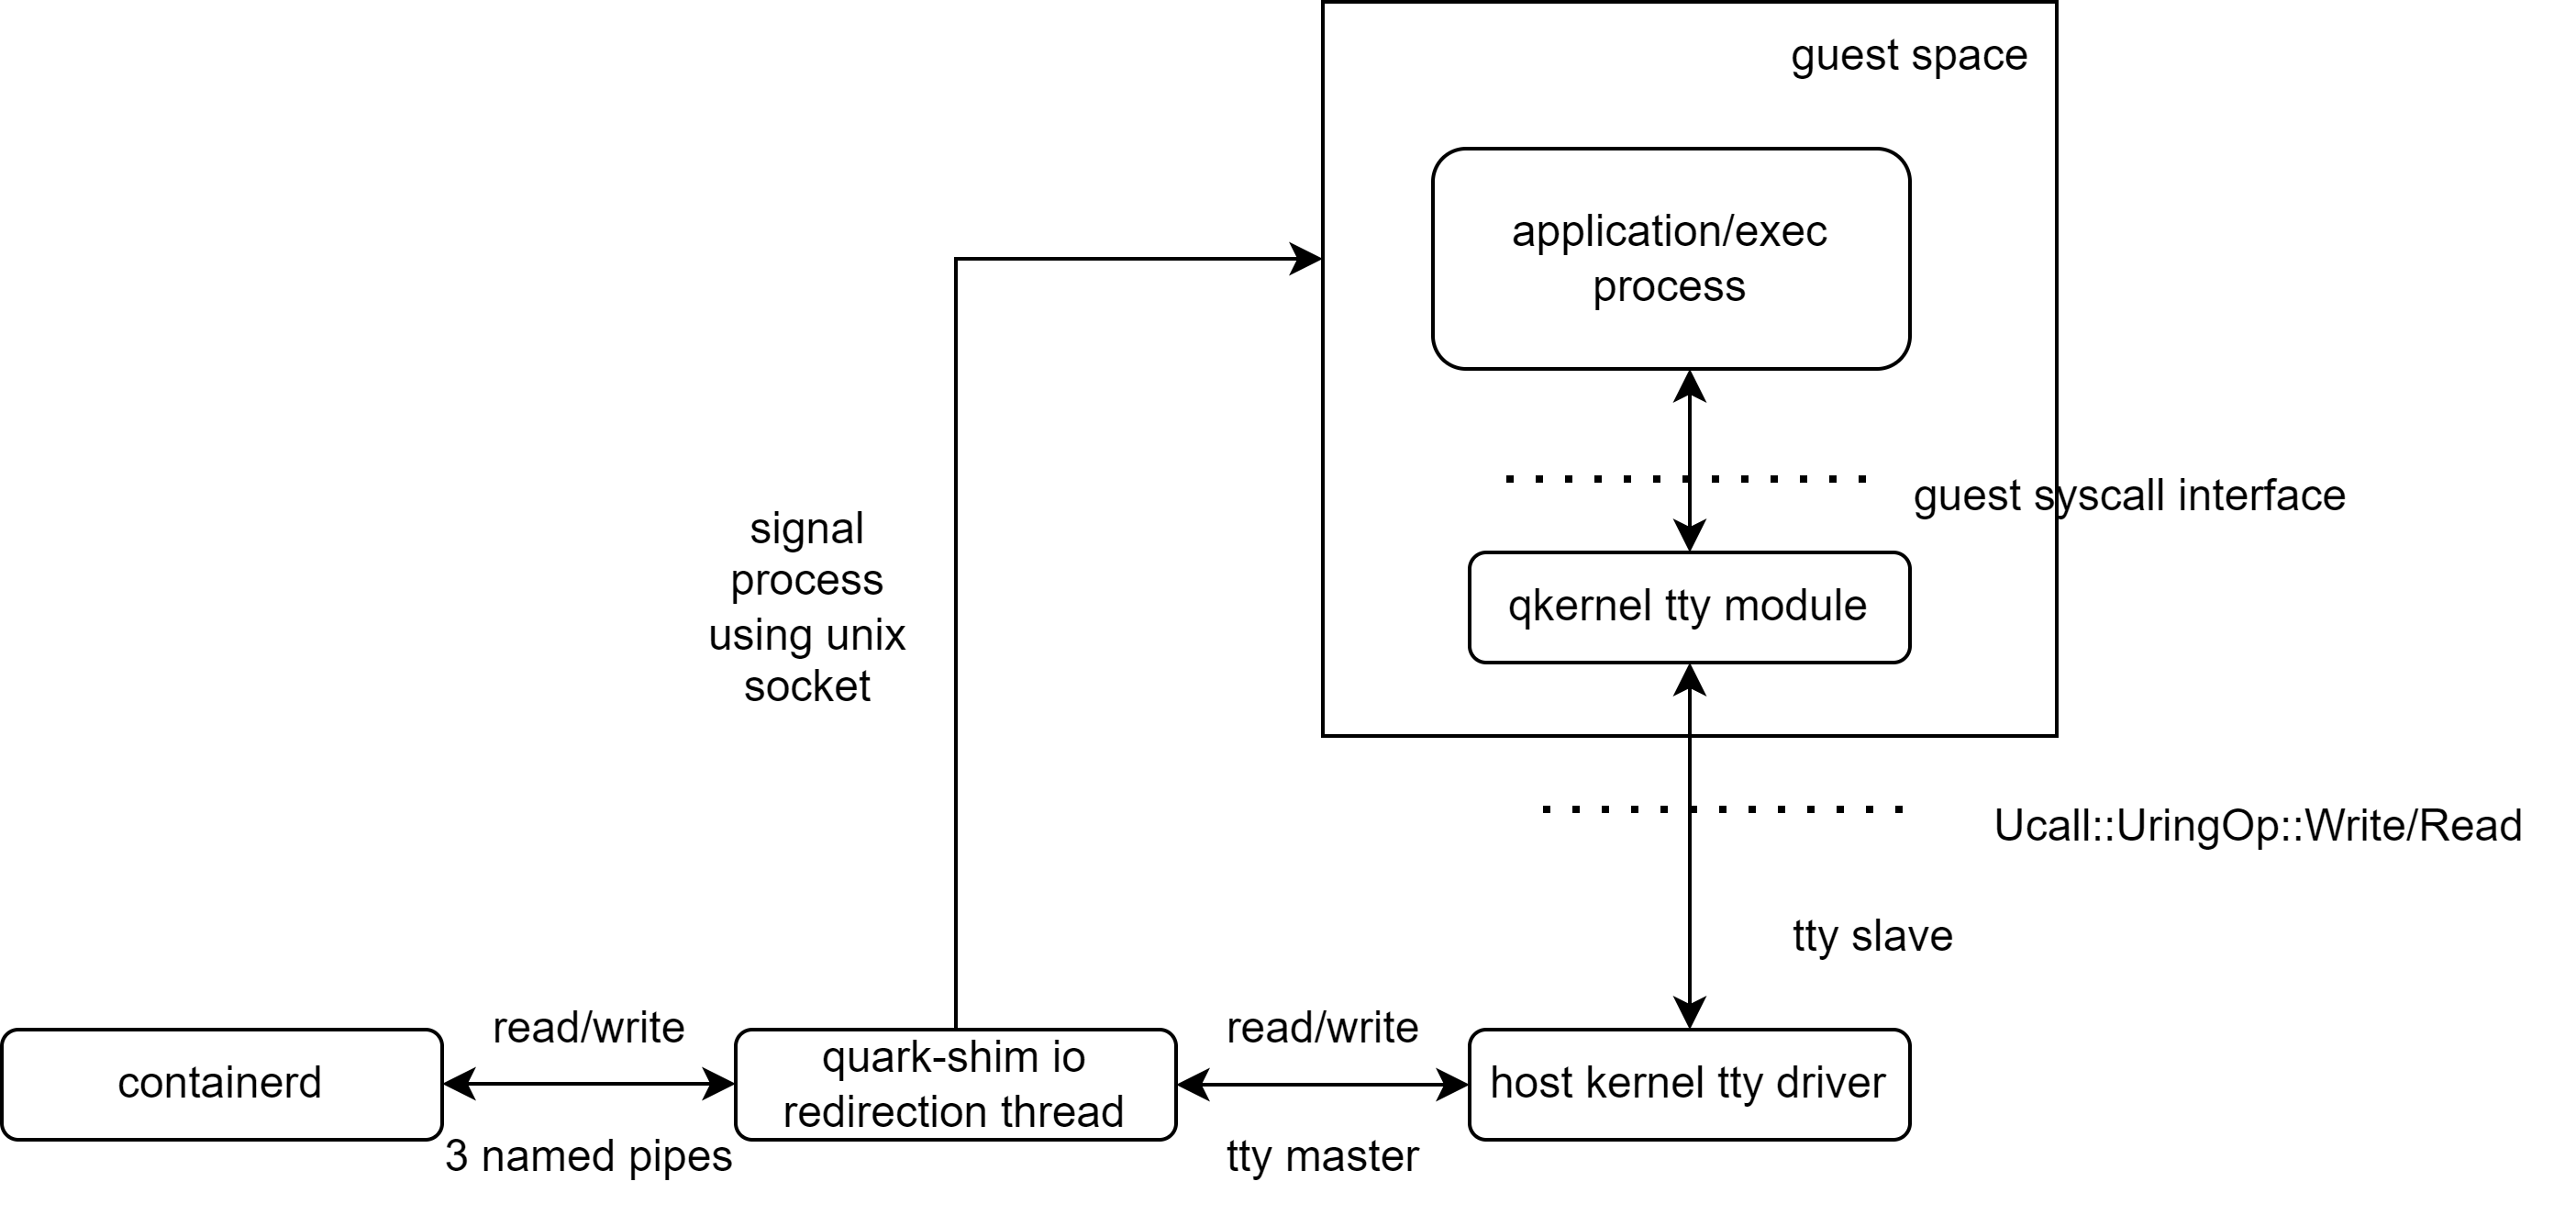
\includegraphics[width=0.9\linewidth]{images/termianl_workflow.png} 
      \caption{Terminal IO} 
      \label{fig1:b} 
      \vspace{4ex}
    \end{subfigure} 
    \caption{Guest User Space Process STDIO Handling Workflow}
    \label{fig1} 
\end{figure}


The Quark handles the process’s STDIO differently based on the terminal keyword in the specification. 
 
The terminal keyword is true for an interactive process. In this case, as illustrated in Figure~\ref{fig1:b}, Quark Shim creates an asynchronous terminal IO redirection thread and requests a TTY pair from the host kernel (TTY master and TTY slave). The TTY 
slave is then sent to the Quark agent, where it is set as STDIN, STDOUT, and STDERR of the process. The Qkernel TTY module can read and write the TTY slave through the UCLL interface. Furthermore, the redirection thread filters the signals in the STDIN-named pipe and 
transfers the data between the TTY master and the named pipes. The filtered signals include SIGINT, SIGQUIT, and SIGTSTP, which are forwarded to the Quark agent via the Unix socket. In this case, the Quark agent will signal the process accordingly. For instance, when the character \textasciicircum C (ASCII code 3) appears in 
the STDIN-named pipe, the redirection thread sends SIGINT to the process, ultimately terminating it. Besides, the data written to the TTY master and slave are processed by the host kernel TTY drive. For data written to the slave, the driver translates each line feed (\textbackslash n) into a carriage return
followed by a line feed (\textbackslash r\textbackslash n). This editing is required because the user-side terminal needs these two characters to start a new line of text. Also, for characters written to the TTY master, the driver first echoes them back to the user and stores a copy in an internal buffer. When the user presses the enter key (\textbackslash r) 
it copies the buffered data to the TTY slave. As such, the terminal will not work without the host kernel TTY driver.

The terminal keyword is false for a non-interactive process. In this case, as shown in Figure~\ref{fig1:a}, Quark Shim directly sends the three named pipes to the Quark agent. It then creates the process and uses the pipes as STDIN, STDOUT, and STDERR. 
Unlike the former case, Qkernel uses the Qcall interface for STDIO data transmission.

While the process is running, Containerd~\cite*{containerd} will keep the three named pipes open. For the application process, STDOUT and STDERR stream output is saved as container logs to a location specified by Kubernetes\cite*{k8s}. For an EXEC process, the command execution result is returned to the user via 
STDOUT or STDERR.

% In computer security, the man-in-the-middle 
% attack~\cite*{Man_in_the_middle_attack} is a common attack mode where an attacker can intercept and forward messages between two parties to eavesdrop or alter communications. In the case of Quark,  Quark Shim, as a man-in-the-middle, can intercept confidential data when redirecting the data between the TTY master and the named 
% pipes. 

\textbf{Lack of cryptographic protection for interactive processes STDIN, STDOUT, and STDERR}. Firstly, if the application owner uses a terminal to communicate with an interactive process, the integrity and confidentiality of transmitted data may be compromised.  
This is because the data is transferred through untrusted entities such as containerd, Quark Shim, and the host kernel. Besides, the log of the interactive application is managed by Kubernetes. An individual with cluster access can use the” kubectl logs pod-name” to view the application logs. To this end, the interactive processes STDIN, STDOUT, and 
STDERR should be encrypted. Specific mitigation measures can be found in Section~\ref{sec:design_STDIO_PROTECTION}.
 
 
\textbf{The STDOUT and STDERR of a non-interactive process require protection for several reasons.} Firstly, the data from a non-interactive application process’s STDERR and STDOUT is stored as logs in the host. This can result in the leakage of confidential data. Additionally, an EXEC process writes the command execution result to its STDOUT. The result is 
redirected by untrusted Qvisor and Containerd~\cite*{containerd} to the user. Since the execution results of commands issued by the application owner may contain sensitive data, we must prevent untrusted entities from accessing them. To this end, we must protect the STDOUT and STDERR of a non-interactive process. The mitigation can be found in 
Section~\ref{sec:design_STDIO_PROTECTION}.


\subsection{Issuing Command and Terminal Allocation}
\textbf{Anyone can use kubectl exec to issue commands to an application.} These include commands that allocate terminals, such as /bin/sh, and others, like cat, etc. The Quark agent (see section~\ref{sec:security_analyse_STDIO} for an explanation) lacks authentication and access control on the EXEC requests sent from the Quark Shim. Therefore, an adversary can 
issue arbitrary commands to an application to collect its secret. For example, an attacker can use kubectl exec pod-name printenv to obtain the application’s environment variable type secrets. To this end, we should add authentication and access control points within Qkernel. Any unauthorized commands should be denied. For further details, please refer to 
section~\ref{sec:design_EXEC_Requests}.


\textbf{The commands issued by the application owner may contain confidential data but are unprotected during transmission.} Currently, the commands are redirected to Qkernel by Containerd~\cite*{containerd} and Quark Shim along with other metadata in EXEC request. When Quark Shim receives an EXEC request, it generates 
a process specification based on the EXEC request’s metadata. This specification includes the command and its parameter, the STDIO type, the environment variables, etc. Quark Shim forwards this specification to the Quark agent via a Unix socket. The Quark agent then creates a guest process to 
execute the command (see Figure~\ref{fig:quark_agent_work_flow}). In this case, the confidentiality and integrity of the commands issued by the application owner may be compromised during transit. To this end, we should apply end-to-end cryptographic protection for these 
commands. For additional information, please see section~\ref{sec:design_EXEC_Requests}.



\textbf{Any user can attach to an application.} Specifically, a user can attach a terminal to an interactive application to issue commands or attach to a non-interactive application to observe its STDOUT stream. Unlike EXEC requests, attach requests are handled by Containerd~\cite*{containerd}. For example, Containerd creates an IO redirection thread that 
transfers data between the STDIO of the terminal and the three named pipes in Containerd representing the application STDIO when it receives the terminal attach request. As such, Qkernel has no control over the request. One possible countermeasure is to encrypt the STDOUT and STDERR of the application. In this case, even if an attacker attaches to the application, he 
can not obtain any useful information because the attacker does not have the key to decrypt the STDOUT and STDERR streams of the application. The mitigation can be found in Section~\ref{sec:design_STDIO_PROTECTION}.

 

\subsection{Paravirtualized File System Sharing}
The application accesses the rootfs on the host through the Paravirtualized File System Sharing mechanism. In creating the application, Quark Shim first generates a mount namespace for the Quark sandbox. It then utilizes the information in the application bundle to mount the rootfs of an application 
into the Quark sandbox path, thus making it available to the Qkernel. During runtime, the application accesses the rootfs on the host through the Qkernel para-virtualized file system. For instance, when the application utilizes the guest-read system call to access a file, the Qkernel will request 
the host to read the target file via Hypercall or Ucall interface. 


\begin{figure}[ht] 
  \begin{subfigure}[b]{0.5\linewidth}
    \centering
    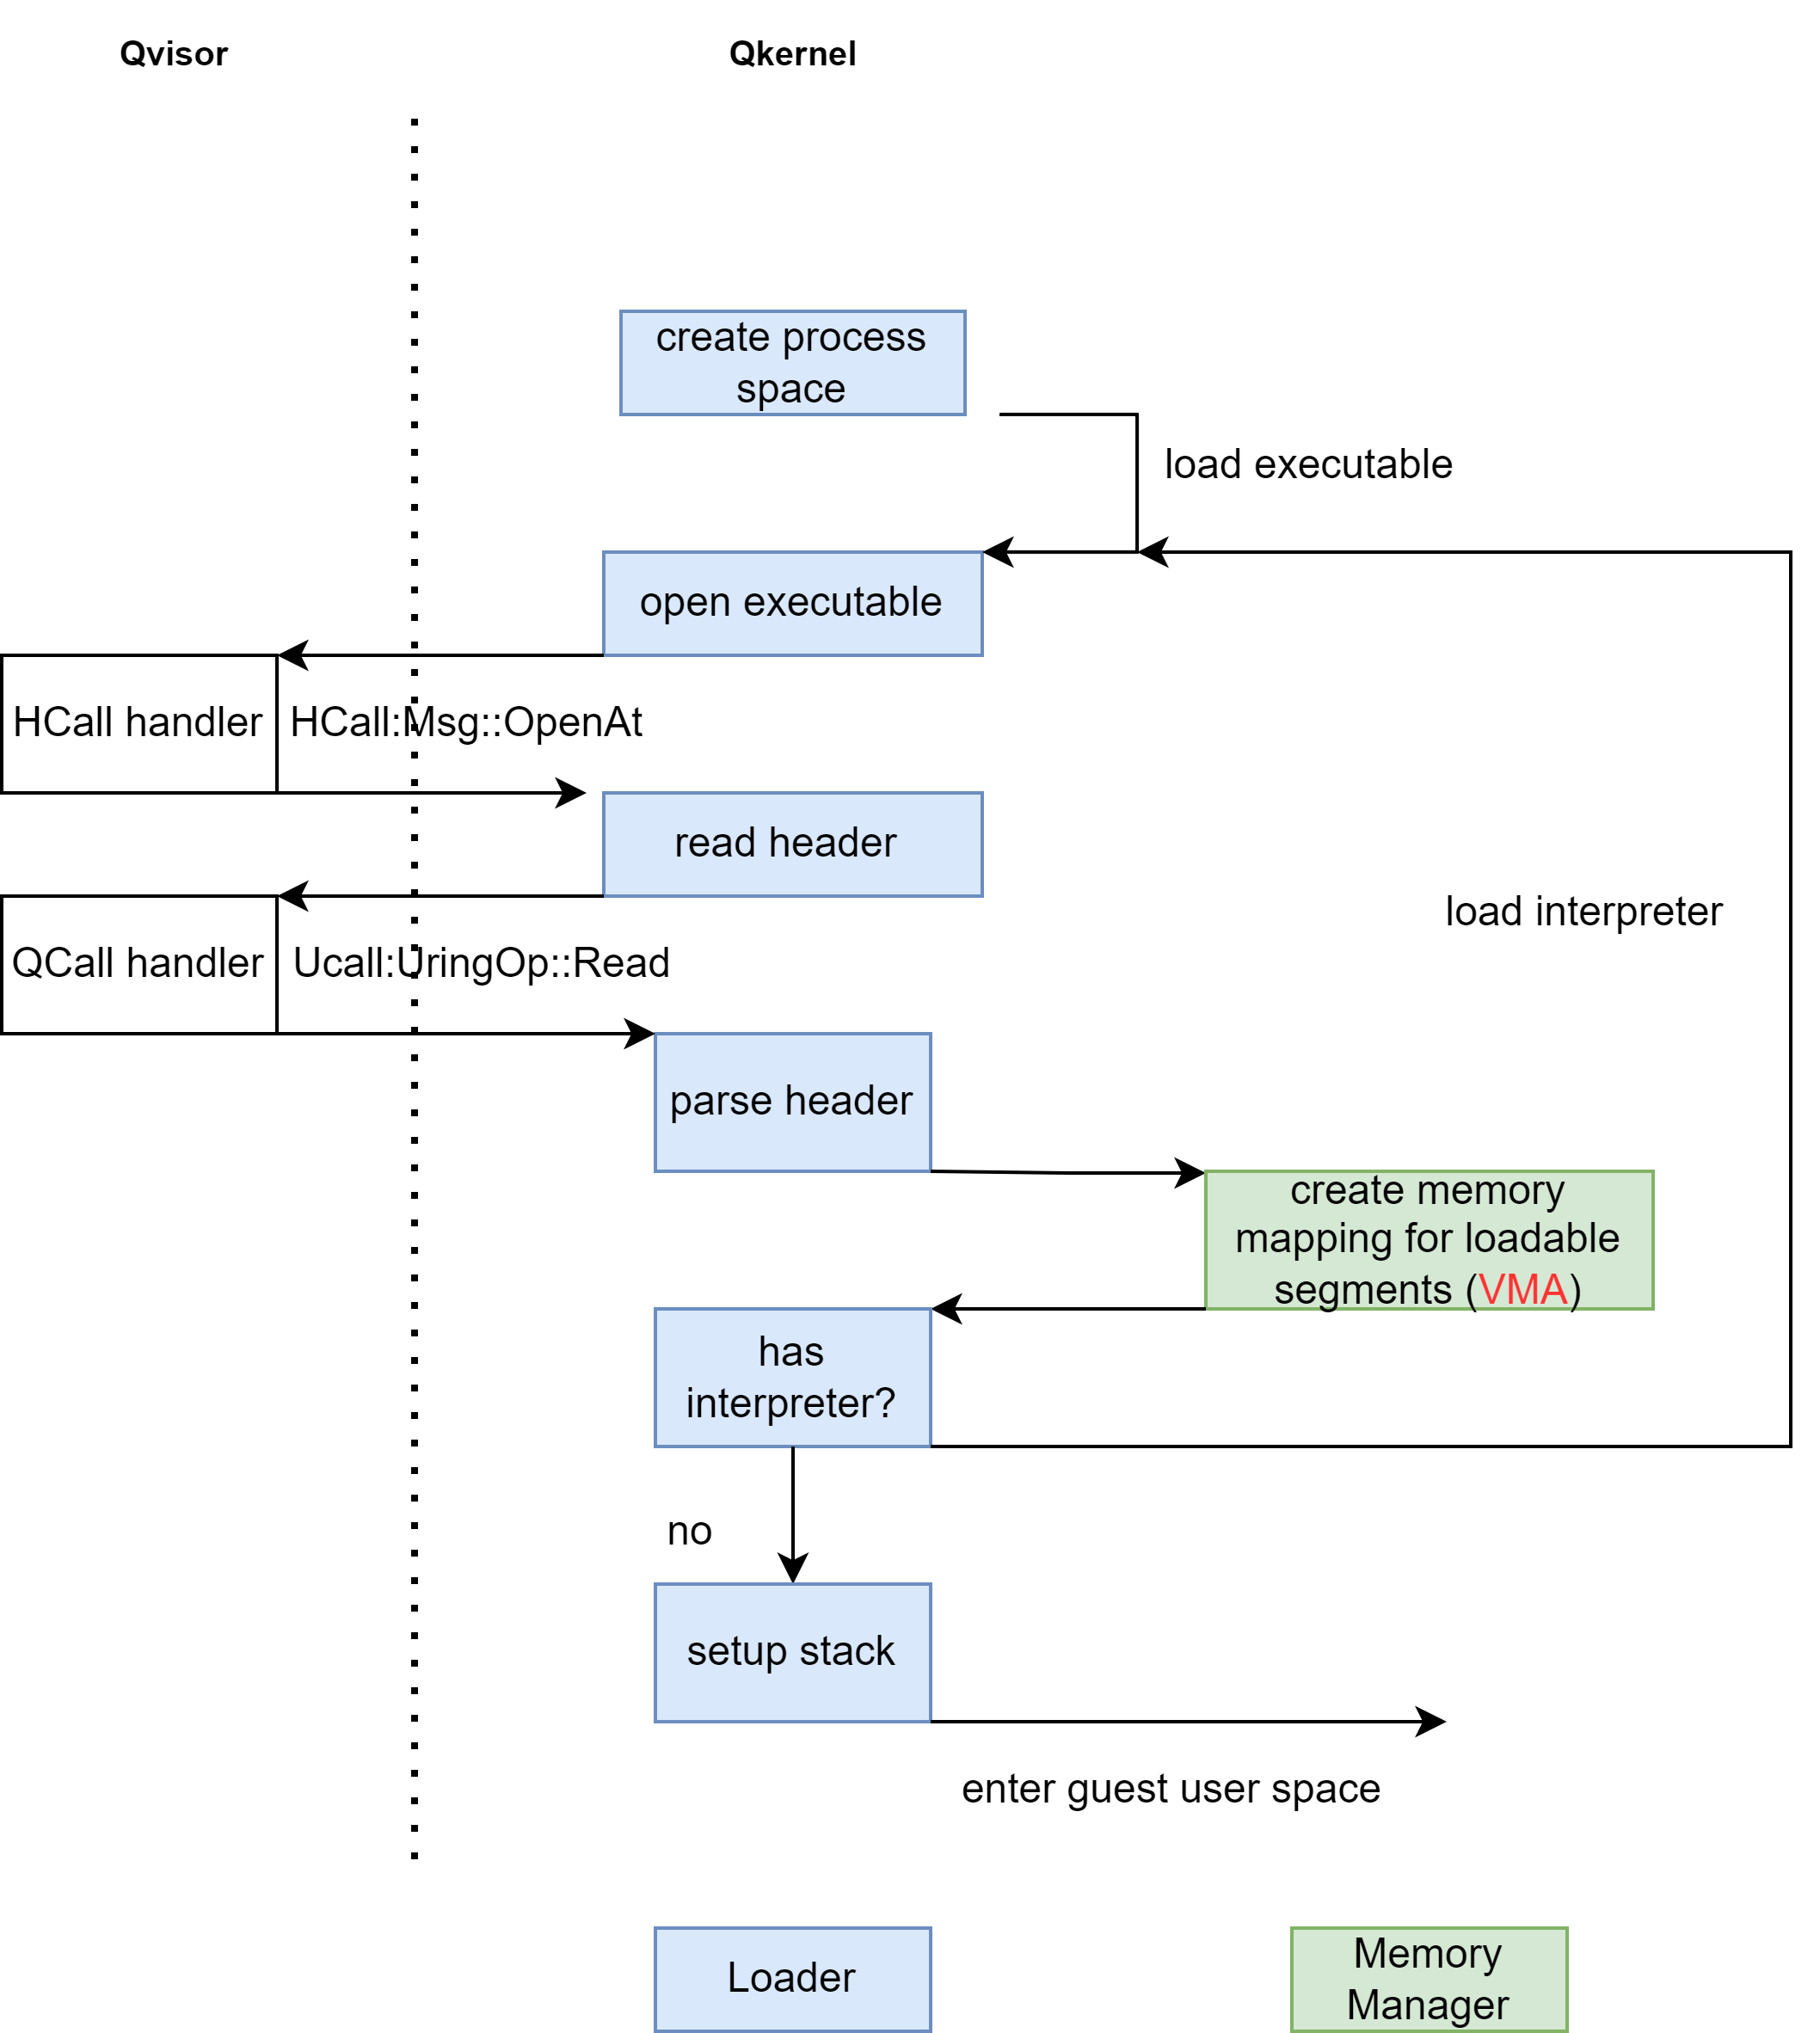
\includegraphics[width=0.9\linewidth]{images/loader_flow.png} 
    \caption{Loader setup memory mappings during application startup} 
    \label{fig2:a} 
    \vspace{4ex}
  \end{subfigure}%% 
  \begin{subfigure}[b]{0.5\linewidth}
    \centering
    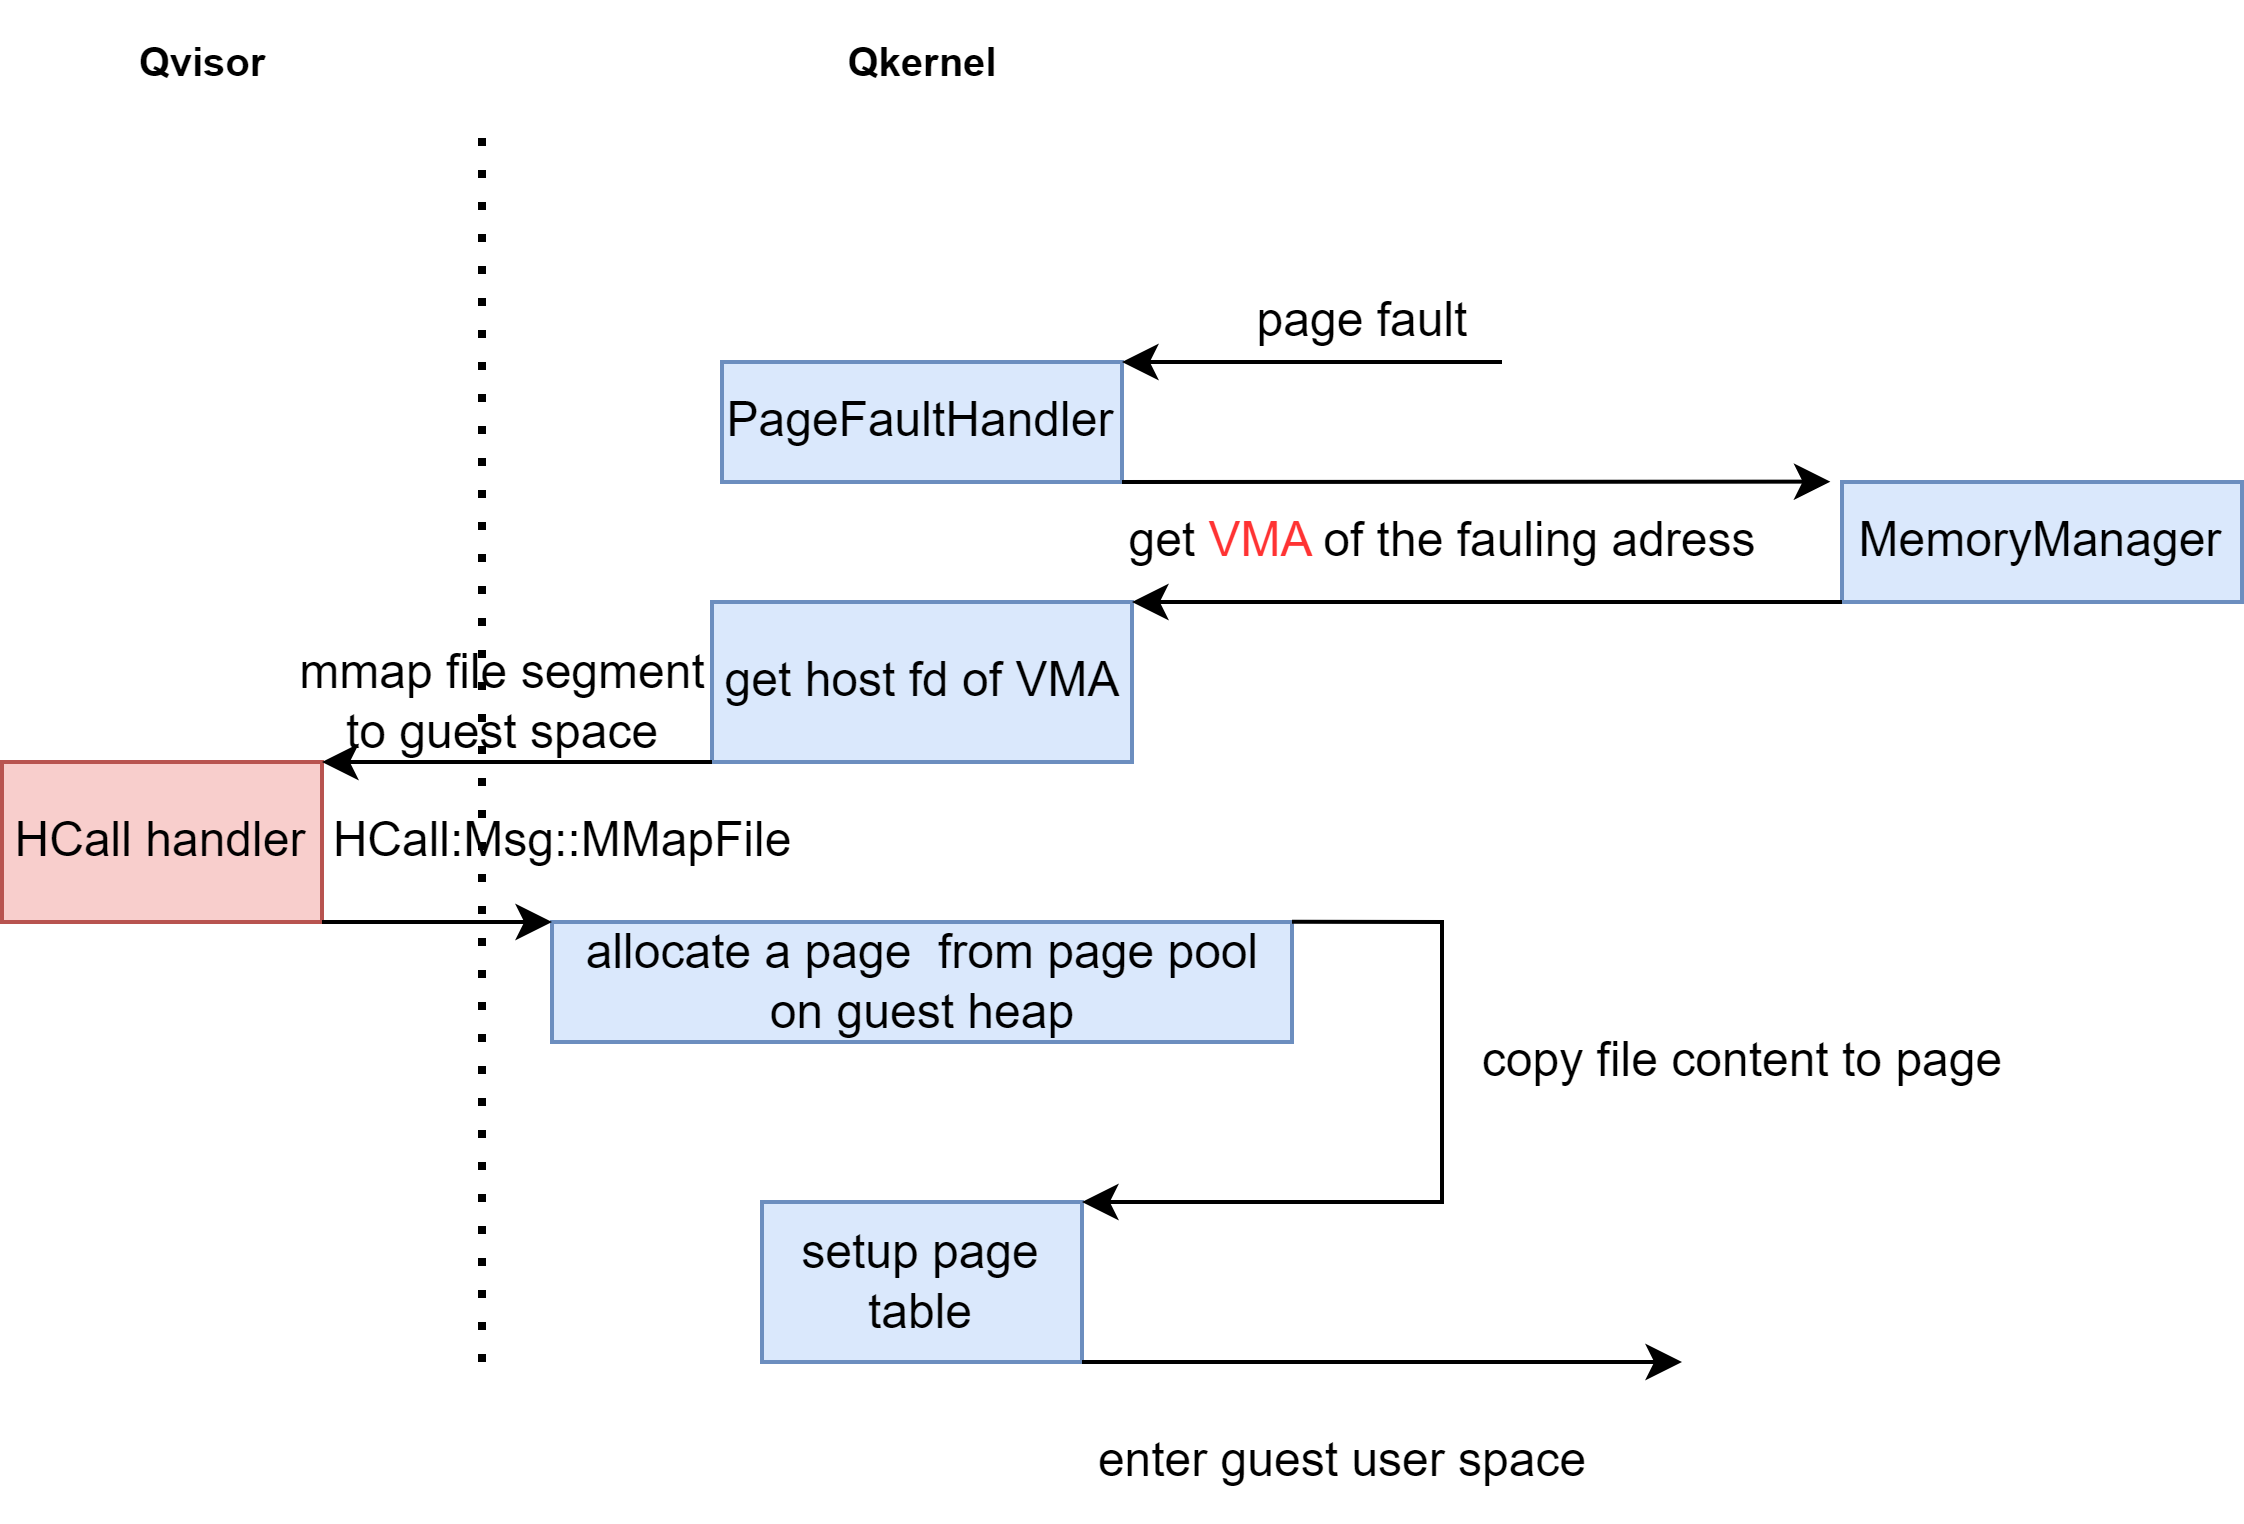
\includegraphics[width=0.9\linewidth]{images/page_fault_handling.png} 
    \caption{Page Fault Handling} 
    \label{fig2:b} 
    \vspace{4ex}
  \end{subfigure} 
  \caption{Application binary loading process}
  \label{fig2} 
\end{figure}

\subsubsection{Loading compromised Application Binary during Startup}
\label{sec:app_binary_loading}
The application binary is stored on the host. During the setup of the application process, the Qkernel loader opens the application binary using Hcall::Openat, reads its ELF header into the Qkernel using the Ucall::read, and then requests the Qkernel virtual memory manager to create a private virtual 
memory area (\acrshort{VMA}) for each loadable segment defined in the ELF file (Figure~\ref{fig2:a}). When the application process runs, accessing an address within the \acrshort{VMA} will trigger a page fault, which is handled by the Qkernel page fault handler.
 
The workflow for the page fault handling can be found in Figure~\ref{fig2:b}. Since the \acrshort{VMA} of a loadable segment is private, the page fault handler uses hcall::mmap to request Qvisor to map the loadable segment into a guest's physical address. It then allocates a page from the page pool on the Qkernel heap and copies the 
segment's contents from the guest's physical address to this page. Finally, a page table entry (guest virtual address -> address of the page) is created. After this, the page fault handler hand over the control to the guest user process.
 
Since the application binary is loaded from the host,  an attacker can induce Qkernel to execute compromised codes. For instance, the loader might request Qvisor to open binary A using Hcall::openat. Nevertheless, instead, Qvisor provides the descriptor of file B. As a result, the loader creates the 
wrong memory mapping. Consequently, the page fault handler will load the code from file B instead of file A. Furthermore, since the page fault handler uses Hcall::mmap to map the executable into the guest's physical space, an attacker could manipulate the Qvisor to map compromised code. In this case, 
the page fault handler copies this code to a page, creates a page table entry, and then returns to the application process without an integrity check.  
 
To this end, the application binary should be loaded to the guest and measured when the Qkernel loader creates the \acrshort{VMA}s for it. The measurements should be forwarded to relying party for integrity checking. Further detail can be found in Section~\ref{sec:Enclave_Runtime_Measurement}. 

\begin{figure}[htp]
  \centering
  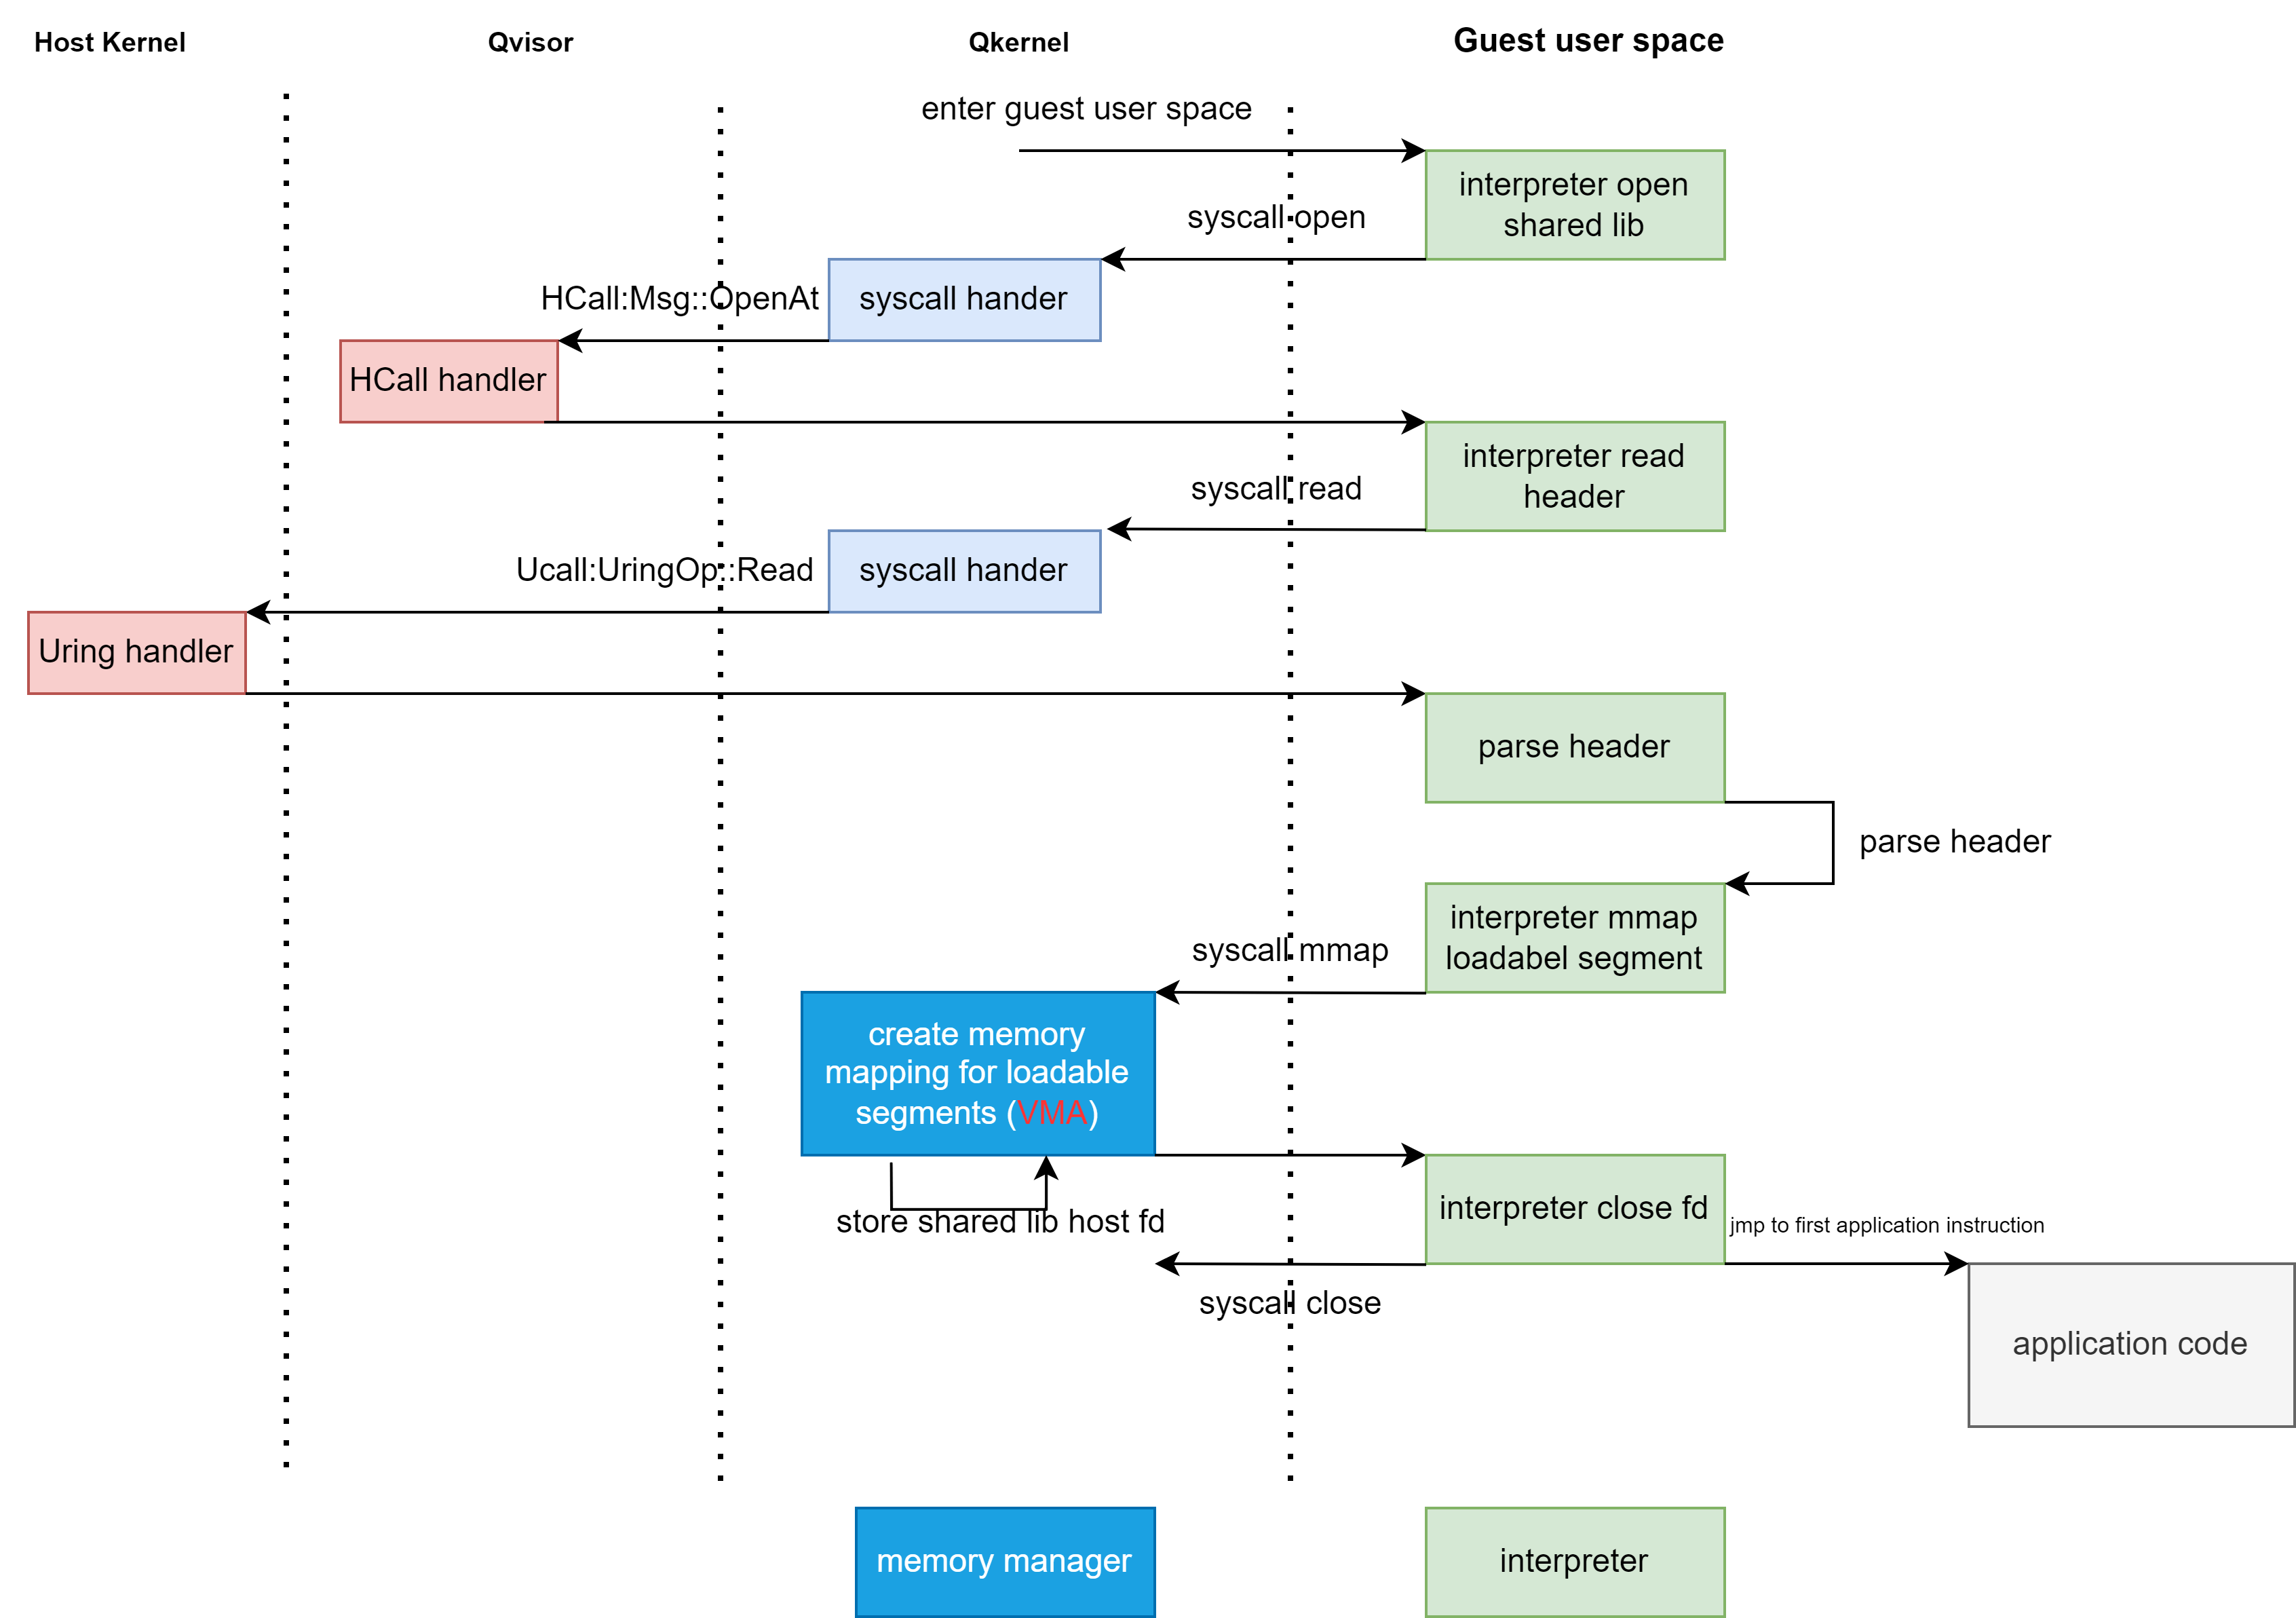
\includegraphics[width=0.6\textwidth]{images/load_shared_libarart.png}
  \caption[Interpreter setups shared library's memory mappings]{Interpreter setups shared library's memory mappings}
  \label{fig:load_shared_libarart}
\end{figure}


\subsubsection{Loading compromised Binary at Runtime}
Dynamic libraries are stored on the host and loaded at application runtime by the interpreter. When the application is a dynamically linked executable, the interpreter's code is executed upon launching the application process. As depicted in Figure~\ref{fig:load_shared_libarart}, the interpreter uses the open, read, and mmap 
system calls to create private memory mappings (\acrshort{VMA}s) for the loadable segments in a shared library. Accessing an address within the \acrshort{VMA}s triggers page faults. The page fault handler handles the fault like how it handles page faults when accessing the \acrshort{VMA} of the application binary.
Since the process of how the Qkernel creates memory mapping and later loads code to the guest for shared libraries and application binary are very similar, the issues encountered in the previous section also apply here. 
 
Executing a command at runtime will cause the Qkernel to load the command binary. The binary loading mechanism has already been discussed in section~\ref{sec:app_binary_loading}. Therefore, a malicious user can inject malicious code into the Qkernel. 
 
Regarding the mitigation, Qkernel should measure the binaries and shared libraries after its \acrshort{VMA} is created and checks its correctness using the reference hashes in the policy file obtained from the relying party. Further detail can be found in Section~\ref{sec:Enclave_Runtime_Measurement}. 


\subsubsection{Lack of Management of Application Restart}
In an unexpected application crash, Kubernetes~\cite*{k8s} may recreate a pod to execute the crashed application or restart the program within the original pod if it still exists~\cite*{k8s}. In the latter case, Qkernel reloads the application binaries from the host and provides the application with the secret 
obtained from relying party during the first startup. An attacker may use this opportunity to inject malicious code into Qkernel. To mitigate this threat, Qkernel should measure the application recreation process and compare the result with the initial 
application startup measurement stored on guest memory. If the two hashes do not match, Qkernel should panic.  Further detail can be found in Section~\ref{sec:Enclave_Runtime_Measurement}. 

\subsection{No restriction to the available System Calls for Applications}
The seccomp section in the OCI runtime specification~\cite*{oci-runtime-spec} defines a way to restrict the available system calls for applications. Unfortunately, Qkernel does not support seccomp~\cite*{seccomp}. 
In this case, a vulnerable system call can be abused to attack the Qkernel and other processes. 
% In computer security, component hijacking~\cite*{DBLP:journals/corr/WuGLD16} is an attack pattern in which an attacker can attack the kernel and other processes by hijacking a process and forcing it to execute a vulnerable system call. 
For example, an attacker can start a malicious EXEC process, which uses a vulnerable system call to steal application secrets stored in Qkernel. To this end, Qkernel should implement a guest system call interceptor and allow the application owner to specify the available system calls for an application. For more details, please refer to 
Section~\ref{sec:design_Interceptor}. 

\subsection{No Control over Guest Kernel Arguments}
\begin{figure}[htp]
  \centering
  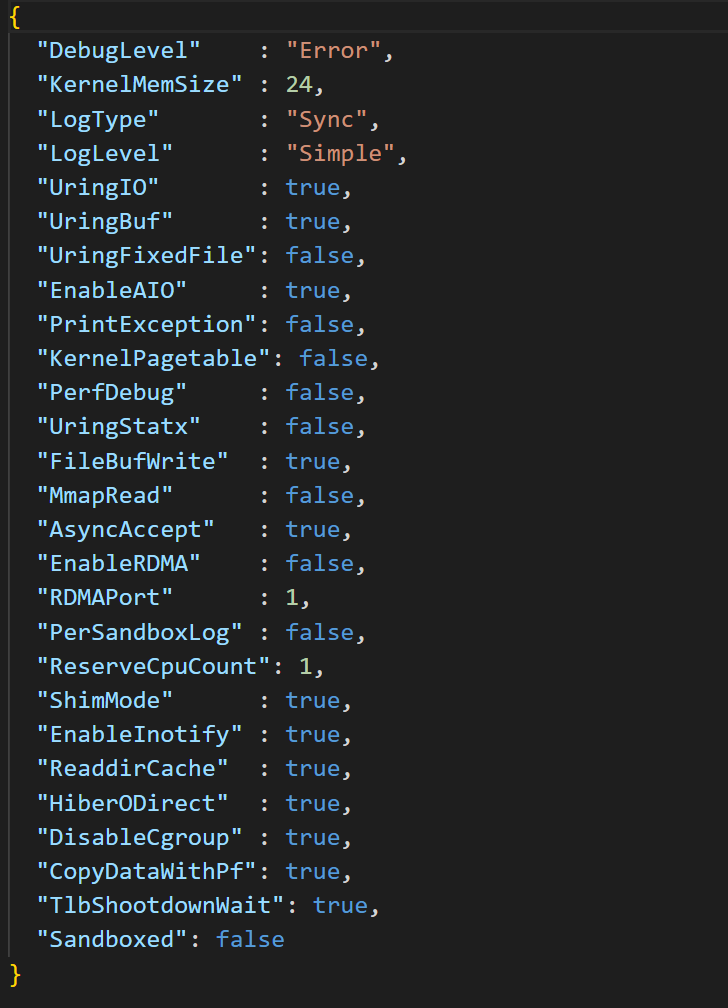
\includegraphics[width=0.3\textwidth]{images/quark_config.PNG}
  \caption[Configuration file for Qkernel, Qvisor, and Quark Shim]{Configuration file for Qkernel, Qvisor, and Quark Shim. The file is installed as a global configuration file for Quark in the /etc/quark/ directory. When Quark Shim or Qvisor starts, it reads this file and completes the relevant configuration}
  \label{fig:quark_config}
\end{figure}

Qkernel is a binary loaded into the guest memory during Qvisor setting up the guest. To properly configure the Qkernel, Qvisor also passes several command-line arguments to the Qkernel, including the number of VCPUs, the socket file descriptor that the Quark-agent listens to, and a configuration 
file shown in Figure~\ref{fig:quark_config}. This configuration file specifies the runtime behavior of the Qkernel, such as whether to enable the Ucall interface, whether to enable RDMA, etc. A wrong configuration file can disclose the secrets stored in Qkernel. For example, turning on RDMA would allow an untrusted 
party direct access to the Qkernel’s memory. For this reason, the Qkernel should measure the configuration file and send it to the relying party for integrity checking. For more details, please refer to section~\ref{sec:Enclave_Runtime_Measurement}.

\subsection{Qkernel Log Misconfiguration}
\label{sec:Qkernel_Log_Misconfiguration}
Qkernel uses Hcall::HYPERCALL\_PRINT to store its logs under the host directory /var/log/quark. The Qkernel logging system supports five logging levels: OFF, Error, Info, Debug, and Trace. Here OFF is the minor level, i.e., the least detailed, and Trace is the highest level, i.e., the most detailed log. The user can configure the highest level of logging for 
Qkernel through the DebugLevel keyword in the configuration file shown in Figure~\ref{fig:quark_config}. For example, when the DebugLevel is Info, Qkernel only prints logs in level Error and Info. 

A malicious administrator may set the DebugLevel keyword to Trace and then analyze the Qkernel logs to obtain sensitive information. This problem can be solved by measuring the guest kernel arguments. However, both Qvisor and Qkernel are configured using this file. Specifically, Qvisor reads this configuration file after startup and passes a copy to the Qkernel when 
launching the guest. In confidential computing, Qkernel and Qvisor belong to the application owner and the cloud provider, respectively. They have different interests and do not trust each other. For example, to resolve errors quickly, the cloud provider requires the log level in Qvisor to be set to TRACE, while the application owner 
requires the log level in Qkernel to be OFF to protect the confidentiality of the \acrshort{CVM}. In the current architecture, Quark cannot satisfy both requirements. To this end, the Qkernel logging system configuration should be offloaded from the global configuration 
file. The detail can be found in section~\ref{sec:Qkernel_logger}.




\section{Summary}
\label{sec:security_summarize}
In this chapter, the threat model is first defined in section~\ref{sec:Threat_model}. Based on this model, the security issues in Quark are examined from various perspectives. These vulnerabilities found include:
\begin{enumerate}
  \item \label{vulnerabilities:1} Application secrets are managed and deployed by untrusted Kubernetes and Quark Shim.
  \item \label{vulnerabilities:2} Lack of cryptographic protection for interactive processes STDIN, STDOUT, and STDERR.
  \item \label{vulnerabilities:3} Lack of cryptographic protection for non-interactive processes STDOUT and STDERR.
  \item \label{vulnerabilities:4} Anyone can issue commands to an application.
  \item \label{vulnerabilities:5} Any user can attach to an application.
  \item \label{vulnerabilities:6} The commands issued by the application owner may contain confidential data but are unprotected during transmission.
  \item \label{vulnerabilities:7} Loading compromised application binary during startup.
  \item \label{vulnerabilities:8} Loading compromised binary/shared library at runtime.
  \item \label{vulnerabilities:9}  Lack of management over application restart.
  \item \label{vulnerabilities:10} No restriction to the available system calls for applications.
  \item \label{vulnerabilities:11} No control over guest kernel arguments.
  \item \label{vulnerabilities:12} Guest kernel log misconfiguration.

\end{enumerate}

% For this reason, we should offload the configuration of the logging system from the qkernel configuration file and allow the application owner to specify the maximum logging level for the specified client kernel logging system in the protection 
% policy.
\cleardoublepage

